
\chapter{Design}

\section{Requirements}

For this project, I will guarantee mutual isolation of tasks' stack and heap memory. Stack-allocated variables in one task shall not be readable nor writable by any other task. Similarly, memory allocated to a task on the heap will not be readable nor writable by any other task (until is freed and reallocated).

This implementation does not support process loading from disk (introduced in lab 5 of EE380L). All tasks are assumed to be compiled with the OS code, as is common for embedded RTOSes.

Importantly, this implementation does not protect task code. Tasks are able to execute any functions that they can be linked against.

Task memory will be protected automatically upon task creation and heap allocation.

As a proof of concept, my implementation can protect memory of up to sixteen different tasks. It cannot scale indefinitely. This is in part due to limitations of the MPU, which imposes a limit on the number of regions that can be individually configured. In a system that must support more tasks, the implementation could be changed to make isolating tasks optional, so that while only sixteen can be protected, more than that may run in the system at any given time.

\section{MPU Functionality}

The MPU is a hardware unit used to protect regions of memory. It supports up to eight configurable memory regions. Each region is configured with a base address, size, and permissions for both privileged and unprivileged access. The region's base address must be aligned to the size of the region. Each region is further divided into eight equally-sized subregions which can be individually enabled or disabled. My design will leverage subregions heavily to maximize the number of tasks that can be mutually isolated.

\section{Stack Protection}

Task stacks are allocated from a pool of statically allocated memory. Sixteen stacks each of 64 double words are declared to be allocated as tasks are created at runtime. Two consecutive MPU regions are initialized to span from the beginning of the stack pool up to the end. Using two regions allows us to evenly divide the pool into sixteen subregions each of which perfectly aligns with the boundaries of a single task stack. Therefore there is a one-to-one correspondence between MPU subregion and task ID. To protect the stack pool with the MPU, the stack pool must be aligned to the size of one of the MPU regions, which is $8\times64$ double words, or 4096 bytes.

\begin{figure}[hbtp]
	\centering
	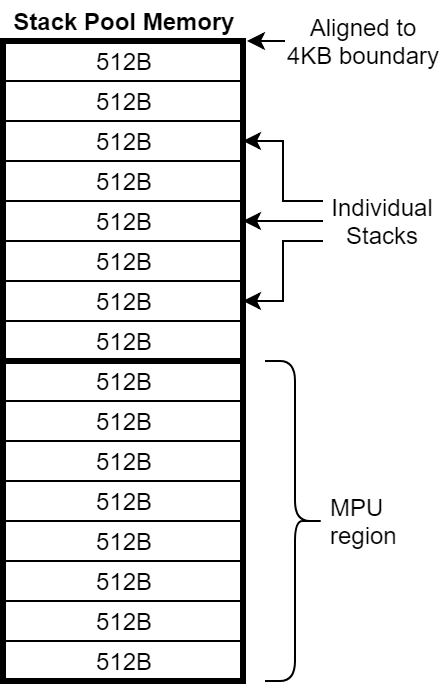
\includegraphics[width=0.4\columnwidth]{figs/stack_prot.png}
	\caption{Illustration of how the stack pool is organized in memory. Two consecutive MPU regions are configured to span the pool. The pool holds sixteen consecutive 512B stacks which each align with a MPU subregion. The whole stack pool is aligned to a 4KB boundary.}
	\label{fig:stack_prot}
\end{figure}

\section{Heap Protection}

\begin{figure}[hbtp]
	\centering
	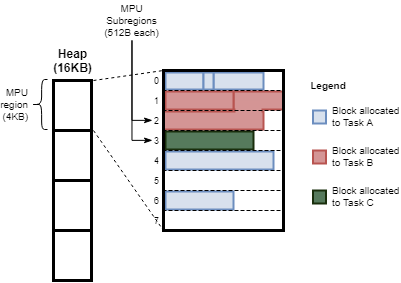
\includegraphics[width=0.8\columnwidth]{figs/heap_prot.png}
	\caption{Illustration of how the heap is organized in memory. Two consecutive MPU regions are configured to span the heap, each with eight subregions. Memory allocated to different tasks will always be placed in different subregions such that every subregion's blocks are associated with at most one task.}
	\label{fig:heap_prot}
\end{figure}

\section{Context Switch}

During a context switch, the OS configures the MPU to allow access only to stack and heap subregions associated with the next running task. All other subregions (either associated with other tasks or unused) are protected.